\begin{figure}[htbp]
\section*{ U2AF2}
\centering
\begin{subfigure}[b]{0.95\textwidth}
\centering
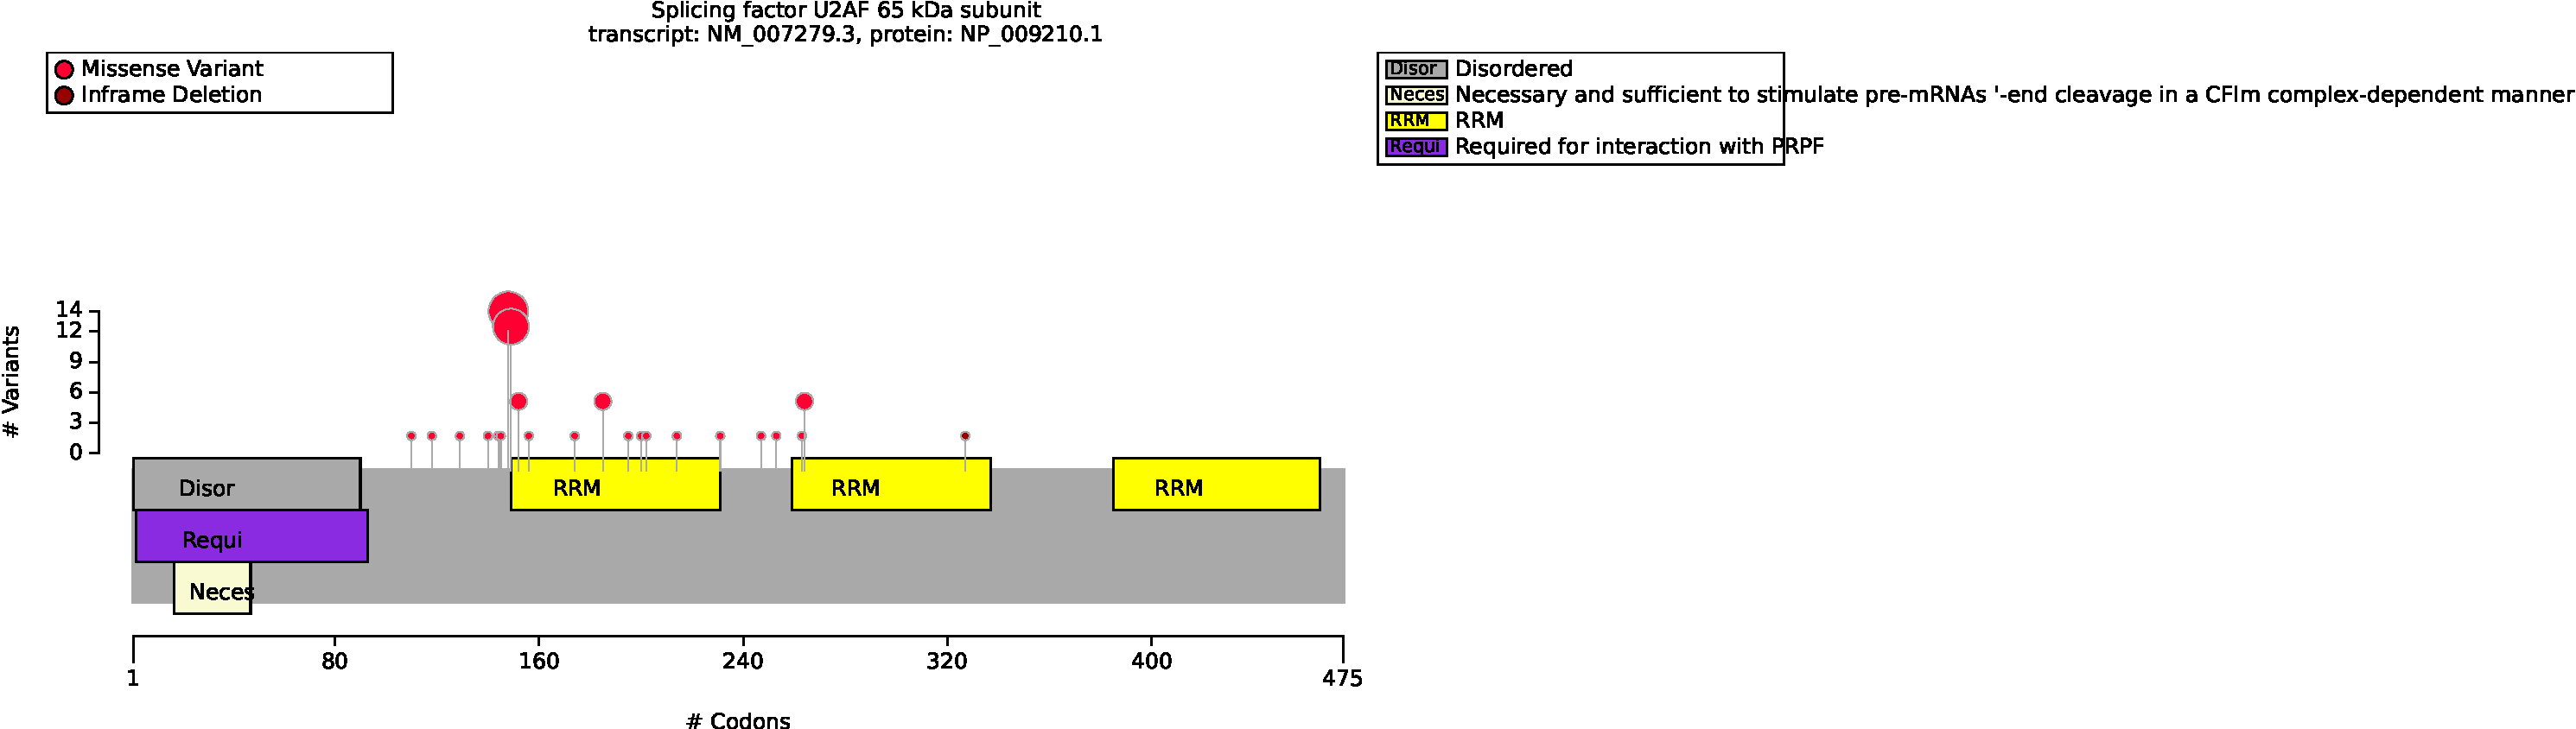
\includegraphics[width=\textwidth]{ img/U2AF2_protein_diagram.pdf} 
\captionsetup{justification=raggedright,singlelinecheck=false}
\caption{Distribution of variants in U2AF2}
\end{subfigure}

\vspace{2em}

\begin{subfigure}[b]{0.95\textwidth}
\centering
\resizebox{\textwidth}{!}{
\begin{tabular}{llllrr}
\toprule
Genotype (A) & Genotype (B) & total tests performed & significant results\\
\midrule
r149W & other & 177 & 0\\
R149,R150 variants & other & 177 & 0\\
RRM 1 & other & 177 & 0\\
FEMALE & MALE & 177 & 0\\
\bottomrule
\end{tabular}
}
\captionsetup{justification=raggedright,singlelinecheck=false}
\caption{Fisher Exact Test performed to compare HPO annotation frequency with respect to genotypes. }
\end{subfigure}

\vspace{2em}

\caption{ The cohort comprised 48 individuals (28 females, 20 males). 2 of these individuals were reported to be deceased. A total of 178 HPO terms were used to annotate the cohort. Disease diagnosis: Developmental delay, dysmorphic facies, and brain anomalies (OMIM:620535). No statistical analysis of GPCs in U2AF2 identified in published literature. A total of 24 unique variant alleles were found in \textit{U2AF2} (transcript: \texttt{NM\_007279.3}, protein id: \texttt{NP\_009210.1}).}
\end{figure}
